The system focuses on simplifying the management of information related to train traveling and ticket payment for its users. The system will provide an account for each user which will store information regarding travel distance, destinations, payments, etc. This will help both users travelling by train and the companies providing the travelling services by keeping track of all these components in a centralized manner. 

The system will present the user with the choice of making an automated payment for each trip through the connection between the mobile app and the beacon in the train cart. Alternatively, an external payment system will be presented to the user I every train station where they can log in and perform the transaction. 

A second important target for our system will be represented by companies providing travelling services by train, which may include governmental institutions or different private companies.

\section{Logical view}

The following diagram displays the main use cases of the system which will be further described in use case scenarios:

\begin{figure}[H]
	\centering
	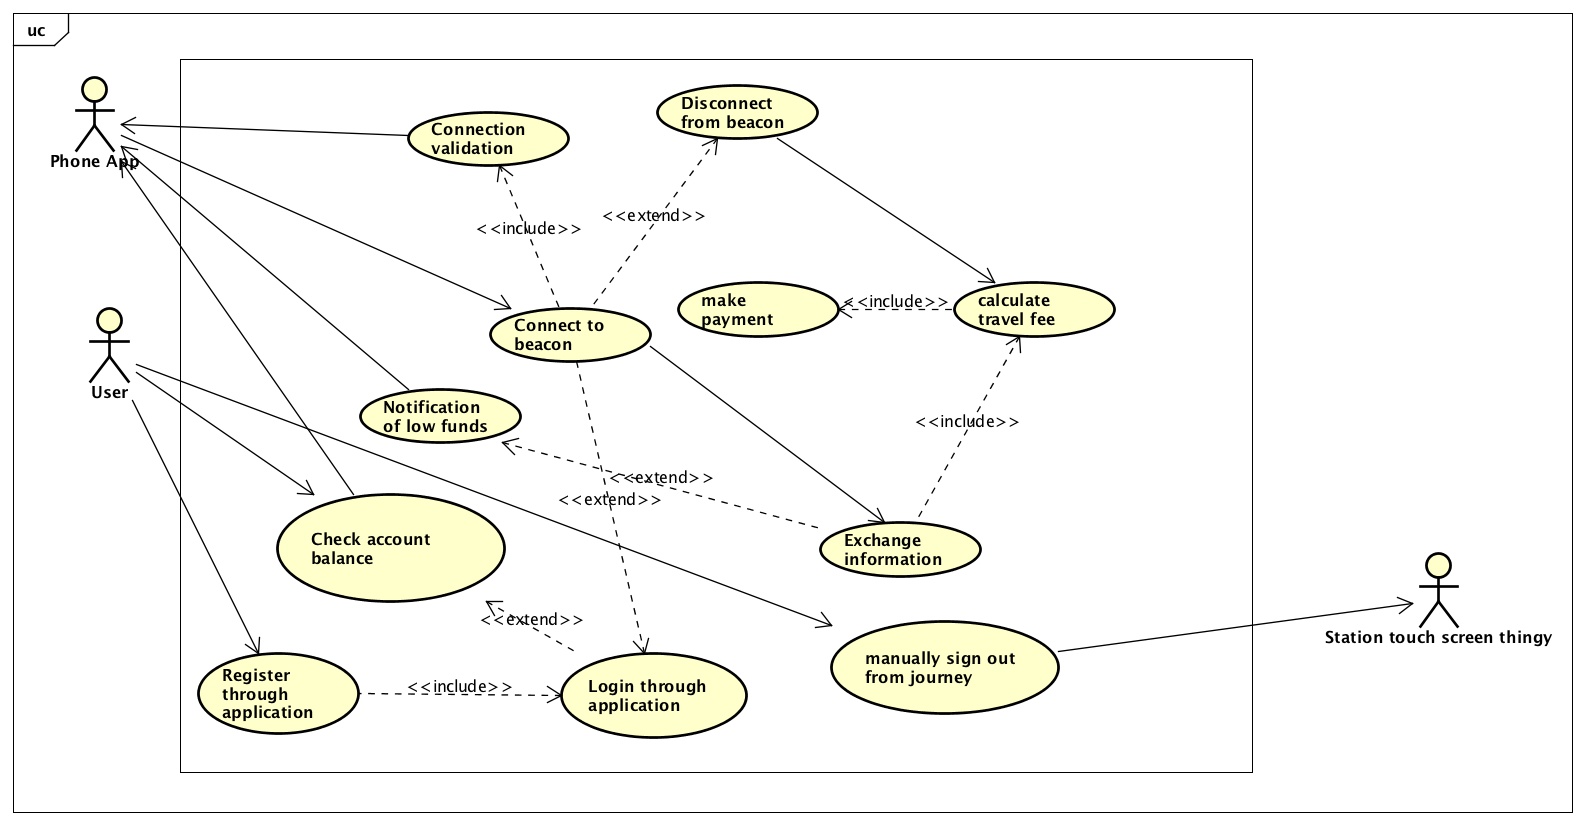
\includegraphics[width=\textwidth]{Pictures/main_use_cases.png}
	\caption{Main use cases}
	\label{fig:main_use_cases}
\end{figure}

\begin{table}[H]
	\centering
	\begin{tabularx}{\linewidth}{l|X}
		\textbf{Usecase}      & Connect phone \\ \hline
		\textbf{Main actor}  & Phone app \\ \hline
		\textbf{Goal}   & Connect to the beacon \\ \hline
		\textbf{Preconditions}     & \begin{itemize}
			\item Bluetooth is switched on
			\item App is installed
			\item Train has left the station
		\end{itemize} \\ \hline
		\textbf{Main scenario}    & \begin{itemize}
			\item The beacon discovers the phone
			\item The phone receives a notification from the beacon
			\item The beacon saves the account information locally
		\end{itemize} \\ \hline
		\textbf{Exception scenarios} & 
		\begin{itemize}
			\item The app doesn’t get the notification because
			the phone is off
			\item The app doesn’t get the notification, due to a
			communication failure 
			\item The beacon fails to detect the phone
			\item The app is installed but the owner doesn't have an account
		\end{itemize}
		\\ \hline
		\textbf{Postconditions} & 
		\begin{itemize}
			\item Phone is connected
			\item Information exchange between phone and beacon
		\end{itemize}
		
		\\ \hline
		\textbf{Related requirements} & NFR2, FR2, NFR3\\ \hline
	\end{tabularx}
	\caption{Main use cases - }
	\label{tbl:uc1}
\end{table}

\begin{table}[H]
	\centering
	\begin{tabularx}{\linewidth}{l|X}
		\textbf{Usecase}      &  \\ \hline
		\textbf{Main actor}  & \\ \hline
		\textbf{Goal}   &  \\ \hline
		\textbf{Precondition}     &  \\ \hline
		\textbf{Main scenario}    &  \\ \hline
		\textbf{Exception scenarios} & \\ \hline
		\textbf{Postconditions} & \\ \hline
		\textbf{Related requirements} & \\ \hline
	\end{tabularx}
	\caption{Main use cases - use case 2}
	\label{tbl:uc2}
\end{table}

\begin{table}[H]
	\centering
	\begin{tabularx}{\linewidth}{l|X}
		\textbf{Usecase}      &  \\ \hline
		\textbf{Main actor}  & \\ \hline
		\textbf{Goal}   &  \\ \hline
		\textbf{Precondition}     &  \\ \hline
		\textbf{Main scenario}    &  \\ \hline
		\textbf{Exception scenarios} & \\ \hline
		\textbf{Postconditions} & \\ \hline
		\textbf{Related requirements} & \\ \hline
	\end{tabularx}
	\caption{Main use cases - use case 3}
	\label{tbl:uc3}
\end{table}
